\documentclass[a4paper]{report}
\renewcommand{\thesection}{\arabic{section}}
\usepackage[utf8]{inputenc}
\usepackage{authblk}

% Headers Footers
\usepackage[a4paper,width=170mm,top=20mm,bot=1mm]{geometry}
\usepackage{fancyhdr,ragged2e}
% Header
\fancyhead{}
\lhead{\parbox[t]{0.45\textwidth}{\RaggedRight\rightmark\strut}}
\rhead{\parbox[t]{0.45\textwidth}{\RaggedLeft\leftmark\strut}}
\setlength{\headheight}{1\baselineskip}
\pagestyle{fancy}

% Icons
\usepackage{fontawesome}

% Section Titles
\usepackage{titlesec}
\titlespacing*{\section}
{0pt}{1pt}{1.5pt}
\titlespacing*{\subsection}
{0pt}{1pt}{1.5pt}

% For diagrams
\usepackage{svg}
\usepackage{pgf}
% Box
\usepackage[utf8]{inputenc}
\usepackage{verbatim}

% C++ code style
\usepackage{listings}
\usepackage{xcolor}
\lstset { %
    language=C++,
    backgroundcolor=\color{black!5}, % set backgroundcolor
    basicstyle=\footnotesize,% basic font setting
}
\def\code#1{\texttt{#1}}

% Images
\usepackage{caption}
\usepackage{subcaption}
\usepackage{float}

% References
\usepackage[colorlinks=true,linkcolor=blue,urlcolor=red]{hyperref}%

\title{Parallel \& Distributed Systems \\ Exercise 4: Reverse Cuthill McKee}
\author[1]{Gonidelis Ioannis}
\author[2]{Zikopis Evangelos}
\affil[1]{Department of Electrical Engineering, AUTH, AEM: 8794}
\affil[2]{Department of Electrical Engineering, AUTH, AEM: 8808}
\date{September 2020 \bigskip 
\framebox[\linewidth][c]{\faGithub Code Repository : \url{https://github.com/vagzikopis/ReverseCuthillMcKee}}
}



\begin{document}
\maketitle
\section{Introduction}
The Reverse Cuthill McKee (RCM) is an algorithm to permute a sparse matrix that has a symmetric sparsity pattern into a band matrix form with a small bandwidth. RCM is an alternated form of the Cuthill–McKee algorithm (CM). Both algorithms generate an R set of vertices, that represents the new order of the final graph's vertices. Their difference is that RCM reverses the resulting indexes in R. As we can see in Figure \ref{fig:d1}, the final constructed graph is identical with the initial and their only difference is the node labelling. \par
\bigbreak


\section{Sequential Implementation}
Our sequential implementation was designed based upon the algorithm's steps. The first step was to construct the initial graph from the input sparse matrix. This process is  implemented by the function \code{initializeGraph()}, that generates a \code{Graph *} structure which represents the initial graph. After the graph construction, \code{rcm()} function performs the Reverse Cuthill McKee algorithm. At first, the nodes of the graph are sorted according to their degree. Also, each node's neighbours are sorted according to their degrees. After the sorting step, the node picking process begins were nodes are picked either from the graph or the Q set. For the selected node it is examined whether it should be added to the R set or not. Also, the neighbours of the selected node are added to Q set, if they are not already in. The algorithm ends when all nodes of the graph are placed in the R set. The final step consists of reversing the indexes in R set.

\emph{The next steps of our program are optional, since R set is computed and the algorithm has been completed}. The final graph, that is associated with the output matrix, is constructed by the function \code{finalizeGraph()} and based upon the R set. Finally, the output matrix is constructed by the \code{graphToSparseMatrix()} function. Please note that the last two functions  do not belong to the main computation algorithm, rather that they facilitate the final representation of the matrix. They don't have anything to do with the main algorithmic steps and that's why we won't demonstrate any optimizations on them in this report.
\begin{figure}[H]
  \centering
  \includesvg{diagram}
  \caption{Workflow Diagram}
  \label{fig:d1}
\end{figure}


\section{Parallel Implementation}
Our parallel implementation utilizes the parallelization directives offered by \code{openMP}. There are certain points that need to be addressed first, though. We will try to break the theoretical algorithm into ``computationally heavy" core parts and disambiguate which ones could boost performance when parallelized.

\bigbreak 

\subsection{Graph Initialization}
The reader should notice that this is where the main computation takes place. The two functions that accomplish the Graph Initialization are \code{initializeGraph()} and \code{parallelInitGraph()} for the sequential and the parallel part correspondingly.The reason why this is a heavy process in our program, is because \textbf{we provide the graph along with the degree information for every node}. That is to say, along with the initialization, there is being implemented the core job of counting the number of neighbours for every node. This double loop is distributed in a ``one thread per node" form. Now this is the basic double loop that is parallelizable in our program and that is why it boosts performance the most, when handled properly.
\bigbreak 

\subsection{Quick-Sorting and Picking Nodes}
The main algorithm involves picking nodes from a sorted list. So we have the `sorting' part and the `picking' part. 

Sorting is implemented using \code{quicksort} simply because ``it's quick". There are two important arguments that need to be addressed here. First of all, \code{qsort()} adds a serious amount of overhead when parallelized. We have tried parallelizing it but the performance boost takes place for a minimum of a very high number of nodes. Why not use some more parallelizable sorting algorithm, then? We have tried switching to \code{mergesort}, as it is obvious that is by far more easy to be parallelized. Indeed the speed-up  was greater, when \code{mergesort} was used. But that wasn't our final choice, simply because our ultimate goal was the total performance overall. Creating a fast sequential code in the first place beats creating a slow sequential algorithm just to demonstrate some acceleration skills. To conclude, our code uses \code{quicksort} just because it is faster in every case while our final goal was to make a fast algorithm even faster, by utilizing \code{openMP}. 

On the `picking' part, this is where the nodes are being picked one by one from the queue - \textit{Q} while the very same queue is being filled with each node's neighbours at every iteration. This is just another double loop but there is a catch. The outer loop works in a conditional \code{while()} form and thus waits for a flag variable to reach a proper value, not knowing the number of iterations. This stems from the nature of the algorithm and that is why it can't be parallelized in a performance boost way.

Another important part of this double loop is that we write in the main array \textit{R} and the intermediate queue \textit{Q}. Trying to do this job asynchronously imposes serious restrictions on critical parts of the code. This is because every node inserted does not have a predefined spot (in a form of chunk), rather than its place is decided dynamically according to the previous node (this is true for both nodes and neighbours positioning).\textit{Race conditions} that add significant overhead, appear upon parallelization of the process described above.
\bigbreak 

\subsection{Overall}
From all the above, we could safely conclude, that according to our experiments, parallelizing a single \code{for-loop} of size \code{n} does not offer significant improvements and that is why we avoided it. This is depicted in Figure \ref{fig:parallelism}. There are only two double (and thus time consuming) loops in the (main) program, from which only one is offered for optimization. As one could observe from the test results though, the outcome is pretty encouraging. By applying the optimizations mentioned above, the execution time decreases more than twice, besides the fact that \textit{the algorithm is pretty strict in sharing variables and race conditions or mutual exclusion cases}.
\bigbreak 


\begin{figure}
    \centering
    %% Creator: Matplotlib, PGF backend
%%
%% To include the figure in your LaTeX document, write
%%   \input{<filename>.pgf}
%%
%% Make sure the required packages are loaded in your preamble
%%   \usepackage{pgf}
%%
%% Figures using additional raster images can only be included by \input if
%% they are in the same directory as the main LaTeX file. For loading figures
%% from other directories you can use the `import` package
%%   \usepackage{import}
%% and then include the figures with
%%   \import{<path to file>}{<filename>.pgf}
%%
%% Matplotlib used the following preamble
%%   \usepackage{fontspec}
%%   \setmainfont{DejaVuSerif.ttf}[Path=/home/evangelos/anaconda3/lib/python3.7/site-packages/matplotlib/mpl-data/fonts/ttf/]
%%   \setsansfont{DejaVuSans.ttf}[Path=/home/evangelos/anaconda3/lib/python3.7/site-packages/matplotlib/mpl-data/fonts/ttf/]
%%   \setmonofont{DejaVuSansMono.ttf}[Path=/home/evangelos/anaconda3/lib/python3.7/site-packages/matplotlib/mpl-data/fonts/ttf/]
%%
\begingroup%
\makeatletter%
\begin{pgfpicture}%
\pgfpathrectangle{\pgfpointorigin}{\pgfqpoint{6.430000in}{1.790000in}}%
\pgfusepath{use as bounding box, clip}%
\begin{pgfscope}%
\pgfsetbuttcap%
\pgfsetmiterjoin%
\definecolor{currentfill}{rgb}{1.000000,1.000000,1.000000}%
\pgfsetfillcolor{currentfill}%
\pgfsetlinewidth{0.000000pt}%
\definecolor{currentstroke}{rgb}{1.000000,1.000000,1.000000}%
\pgfsetstrokecolor{currentstroke}%
\pgfsetdash{}{0pt}%
\pgfpathmoveto{\pgfqpoint{0.000000in}{0.000000in}}%
\pgfpathlineto{\pgfqpoint{6.430000in}{0.000000in}}%
\pgfpathlineto{\pgfqpoint{6.430000in}{1.790000in}}%
\pgfpathlineto{\pgfqpoint{0.000000in}{1.790000in}}%
\pgfpathclose%
\pgfusepath{fill}%
\end{pgfscope}%
\begin{pgfscope}%
\pgfsetbuttcap%
\pgfsetmiterjoin%
\definecolor{currentfill}{rgb}{1.000000,1.000000,1.000000}%
\pgfsetfillcolor{currentfill}%
\pgfsetlinewidth{0.000000pt}%
\definecolor{currentstroke}{rgb}{0.000000,0.000000,0.000000}%
\pgfsetstrokecolor{currentstroke}%
\pgfsetstrokeopacity{0.000000}%
\pgfsetdash{}{0pt}%
\pgfpathmoveto{\pgfqpoint{0.533690in}{0.440340in}}%
\pgfpathlineto{\pgfqpoint{6.243530in}{0.440340in}}%
\pgfpathlineto{\pgfqpoint{6.243530in}{1.562670in}}%
\pgfpathlineto{\pgfqpoint{0.533690in}{1.562670in}}%
\pgfpathclose%
\pgfusepath{fill}%
\end{pgfscope}%
\begin{pgfscope}%
\pgfpathrectangle{\pgfqpoint{0.533690in}{0.440340in}}{\pgfqpoint{5.709840in}{1.122330in}}%
\pgfusepath{clip}%
\pgfsetroundcap%
\pgfsetroundjoin%
\pgfsetlinewidth{0.803000pt}%
\definecolor{currentstroke}{rgb}{0.800000,0.800000,0.800000}%
\pgfsetstrokecolor{currentstroke}%
\pgfsetdash{}{0pt}%
\pgfpathmoveto{\pgfqpoint{1.265116in}{0.440340in}}%
\pgfpathlineto{\pgfqpoint{1.265116in}{1.562670in}}%
\pgfusepath{stroke}%
\end{pgfscope}%
\begin{pgfscope}%
\definecolor{textcolor}{rgb}{0.150000,0.150000,0.150000}%
\pgfsetstrokecolor{textcolor}%
\pgfsetfillcolor{textcolor}%
\pgftext[x=1.265116in,y=0.343118in,,top]{\color{textcolor}\sffamily\fontsize{10.000000}{12.000000}\selectfont 5000}%
\end{pgfscope}%
\begin{pgfscope}%
\pgfpathrectangle{\pgfqpoint{0.533690in}{0.440340in}}{\pgfqpoint{5.709840in}{1.122330in}}%
\pgfusepath{clip}%
\pgfsetroundcap%
\pgfsetroundjoin%
\pgfsetlinewidth{0.803000pt}%
\definecolor{currentstroke}{rgb}{0.800000,0.800000,0.800000}%
\pgfsetstrokecolor{currentstroke}%
\pgfsetdash{}{0pt}%
\pgfpathmoveto{\pgfqpoint{2.208891in}{0.440340in}}%
\pgfpathlineto{\pgfqpoint{2.208891in}{1.562670in}}%
\pgfusepath{stroke}%
\end{pgfscope}%
\begin{pgfscope}%
\definecolor{textcolor}{rgb}{0.150000,0.150000,0.150000}%
\pgfsetstrokecolor{textcolor}%
\pgfsetfillcolor{textcolor}%
\pgftext[x=2.208891in,y=0.343118in,,top]{\color{textcolor}\sffamily\fontsize{10.000000}{12.000000}\selectfont 10000}%
\end{pgfscope}%
\begin{pgfscope}%
\pgfpathrectangle{\pgfqpoint{0.533690in}{0.440340in}}{\pgfqpoint{5.709840in}{1.122330in}}%
\pgfusepath{clip}%
\pgfsetroundcap%
\pgfsetroundjoin%
\pgfsetlinewidth{0.803000pt}%
\definecolor{currentstroke}{rgb}{0.800000,0.800000,0.800000}%
\pgfsetstrokecolor{currentstroke}%
\pgfsetdash{}{0pt}%
\pgfpathmoveto{\pgfqpoint{3.152666in}{0.440340in}}%
\pgfpathlineto{\pgfqpoint{3.152666in}{1.562670in}}%
\pgfusepath{stroke}%
\end{pgfscope}%
\begin{pgfscope}%
\definecolor{textcolor}{rgb}{0.150000,0.150000,0.150000}%
\pgfsetstrokecolor{textcolor}%
\pgfsetfillcolor{textcolor}%
\pgftext[x=3.152666in,y=0.343118in,,top]{\color{textcolor}\sffamily\fontsize{10.000000}{12.000000}\selectfont 15000}%
\end{pgfscope}%
\begin{pgfscope}%
\pgfpathrectangle{\pgfqpoint{0.533690in}{0.440340in}}{\pgfqpoint{5.709840in}{1.122330in}}%
\pgfusepath{clip}%
\pgfsetroundcap%
\pgfsetroundjoin%
\pgfsetlinewidth{0.803000pt}%
\definecolor{currentstroke}{rgb}{0.800000,0.800000,0.800000}%
\pgfsetstrokecolor{currentstroke}%
\pgfsetdash{}{0pt}%
\pgfpathmoveto{\pgfqpoint{4.096441in}{0.440340in}}%
\pgfpathlineto{\pgfqpoint{4.096441in}{1.562670in}}%
\pgfusepath{stroke}%
\end{pgfscope}%
\begin{pgfscope}%
\definecolor{textcolor}{rgb}{0.150000,0.150000,0.150000}%
\pgfsetstrokecolor{textcolor}%
\pgfsetfillcolor{textcolor}%
\pgftext[x=4.096441in,y=0.343118in,,top]{\color{textcolor}\sffamily\fontsize{10.000000}{12.000000}\selectfont 20000}%
\end{pgfscope}%
\begin{pgfscope}%
\pgfpathrectangle{\pgfqpoint{0.533690in}{0.440340in}}{\pgfqpoint{5.709840in}{1.122330in}}%
\pgfusepath{clip}%
\pgfsetroundcap%
\pgfsetroundjoin%
\pgfsetlinewidth{0.803000pt}%
\definecolor{currentstroke}{rgb}{0.800000,0.800000,0.800000}%
\pgfsetstrokecolor{currentstroke}%
\pgfsetdash{}{0pt}%
\pgfpathmoveto{\pgfqpoint{5.040217in}{0.440340in}}%
\pgfpathlineto{\pgfqpoint{5.040217in}{1.562670in}}%
\pgfusepath{stroke}%
\end{pgfscope}%
\begin{pgfscope}%
\definecolor{textcolor}{rgb}{0.150000,0.150000,0.150000}%
\pgfsetstrokecolor{textcolor}%
\pgfsetfillcolor{textcolor}%
\pgftext[x=5.040217in,y=0.343118in,,top]{\color{textcolor}\sffamily\fontsize{10.000000}{12.000000}\selectfont 25000}%
\end{pgfscope}%
\begin{pgfscope}%
\pgfpathrectangle{\pgfqpoint{0.533690in}{0.440340in}}{\pgfqpoint{5.709840in}{1.122330in}}%
\pgfusepath{clip}%
\pgfsetroundcap%
\pgfsetroundjoin%
\pgfsetlinewidth{0.803000pt}%
\definecolor{currentstroke}{rgb}{0.800000,0.800000,0.800000}%
\pgfsetstrokecolor{currentstroke}%
\pgfsetdash{}{0pt}%
\pgfpathmoveto{\pgfqpoint{5.983992in}{0.440340in}}%
\pgfpathlineto{\pgfqpoint{5.983992in}{1.562670in}}%
\pgfusepath{stroke}%
\end{pgfscope}%
\begin{pgfscope}%
\definecolor{textcolor}{rgb}{0.150000,0.150000,0.150000}%
\pgfsetstrokecolor{textcolor}%
\pgfsetfillcolor{textcolor}%
\pgftext[x=5.983992in,y=0.343118in,,top]{\color{textcolor}\sffamily\fontsize{10.000000}{12.000000}\selectfont 30000}%
\end{pgfscope}%
\begin{pgfscope}%
\definecolor{textcolor}{rgb}{0.150000,0.150000,0.150000}%
\pgfsetstrokecolor{textcolor}%
\pgfsetfillcolor{textcolor}%
\pgftext[x=3.388610in,y=0.153149in,,top]{\color{textcolor}\sffamily\fontsize{10.000000}{12.000000}\selectfont Size - n}%
\end{pgfscope}%
\begin{pgfscope}%
\pgfpathrectangle{\pgfqpoint{0.533690in}{0.440340in}}{\pgfqpoint{5.709840in}{1.122330in}}%
\pgfusepath{clip}%
\pgfsetroundcap%
\pgfsetroundjoin%
\pgfsetlinewidth{0.803000pt}%
\definecolor{currentstroke}{rgb}{0.800000,0.800000,0.800000}%
\pgfsetstrokecolor{currentstroke}%
\pgfsetdash{}{0pt}%
\pgfpathmoveto{\pgfqpoint{0.533690in}{0.480936in}}%
\pgfpathlineto{\pgfqpoint{6.243530in}{0.480936in}}%
\pgfusepath{stroke}%
\end{pgfscope}%
\begin{pgfscope}%
\definecolor{textcolor}{rgb}{0.150000,0.150000,0.150000}%
\pgfsetstrokecolor{textcolor}%
\pgfsetfillcolor{textcolor}%
\pgftext[x=0.348102in,y=0.428174in,left,base]{\color{textcolor}\sffamily\fontsize{10.000000}{12.000000}\selectfont 0}%
\end{pgfscope}%
\begin{pgfscope}%
\pgfpathrectangle{\pgfqpoint{0.533690in}{0.440340in}}{\pgfqpoint{5.709840in}{1.122330in}}%
\pgfusepath{clip}%
\pgfsetroundcap%
\pgfsetroundjoin%
\pgfsetlinewidth{0.803000pt}%
\definecolor{currentstroke}{rgb}{0.800000,0.800000,0.800000}%
\pgfsetstrokecolor{currentstroke}%
\pgfsetdash{}{0pt}%
\pgfpathmoveto{\pgfqpoint{0.533690in}{0.963091in}}%
\pgfpathlineto{\pgfqpoint{6.243530in}{0.963091in}}%
\pgfusepath{stroke}%
\end{pgfscope}%
\begin{pgfscope}%
\definecolor{textcolor}{rgb}{0.150000,0.150000,0.150000}%
\pgfsetstrokecolor{textcolor}%
\pgfsetfillcolor{textcolor}%
\pgftext[x=0.348102in,y=0.910329in,left,base]{\color{textcolor}\sffamily\fontsize{10.000000}{12.000000}\selectfont 1}%
\end{pgfscope}%
\begin{pgfscope}%
\pgfpathrectangle{\pgfqpoint{0.533690in}{0.440340in}}{\pgfqpoint{5.709840in}{1.122330in}}%
\pgfusepath{clip}%
\pgfsetroundcap%
\pgfsetroundjoin%
\pgfsetlinewidth{0.803000pt}%
\definecolor{currentstroke}{rgb}{0.800000,0.800000,0.800000}%
\pgfsetstrokecolor{currentstroke}%
\pgfsetdash{}{0pt}%
\pgfpathmoveto{\pgfqpoint{0.533690in}{1.445246in}}%
\pgfpathlineto{\pgfqpoint{6.243530in}{1.445246in}}%
\pgfusepath{stroke}%
\end{pgfscope}%
\begin{pgfscope}%
\definecolor{textcolor}{rgb}{0.150000,0.150000,0.150000}%
\pgfsetstrokecolor{textcolor}%
\pgfsetfillcolor{textcolor}%
\pgftext[x=0.348102in,y=1.392485in,left,base]{\color{textcolor}\sffamily\fontsize{10.000000}{12.000000}\selectfont 2}%
\end{pgfscope}%
\begin{pgfscope}%
\definecolor{textcolor}{rgb}{0.150000,0.150000,0.150000}%
\pgfsetstrokecolor{textcolor}%
\pgfsetfillcolor{textcolor}%
\pgftext[x=0.292547in,y=1.001505in,,bottom,rotate=90.000000]{\color{textcolor}\sffamily\fontsize{10.000000}{12.000000}\selectfont Execution Time}%
\end{pgfscope}%
\begin{pgfscope}%
\pgfpathrectangle{\pgfqpoint{0.533690in}{0.440340in}}{\pgfqpoint{5.709840in}{1.122330in}}%
\pgfusepath{clip}%
\pgfsetroundcap%
\pgfsetroundjoin%
\pgfsetlinewidth{1.505625pt}%
\definecolor{currentstroke}{rgb}{1.000000,0.000000,0.000000}%
\pgfsetstrokecolor{currentstroke}%
\pgfsetdash{}{0pt}%
\pgfpathmoveto{\pgfqpoint{0.793228in}{0.492801in}}%
\pgfpathlineto{\pgfqpoint{1.265116in}{0.516374in}}%
\pgfpathlineto{\pgfqpoint{1.737003in}{0.549406in}}%
\pgfpathlineto{\pgfqpoint{2.208891in}{0.609461in}}%
\pgfpathlineto{\pgfqpoint{2.680779in}{0.668823in}}%
\pgfpathlineto{\pgfqpoint{3.152666in}{0.733630in}}%
\pgfpathlineto{\pgfqpoint{3.624554in}{0.831539in}}%
\pgfpathlineto{\pgfqpoint{4.096441in}{0.932003in}}%
\pgfpathlineto{\pgfqpoint{4.568329in}{1.059995in}}%
\pgfpathlineto{\pgfqpoint{5.040217in}{1.180782in}}%
\pgfpathlineto{\pgfqpoint{5.983992in}{1.511655in}}%
\pgfusepath{stroke}%
\end{pgfscope}%
\begin{pgfscope}%
\pgfpathrectangle{\pgfqpoint{0.533690in}{0.440340in}}{\pgfqpoint{5.709840in}{1.122330in}}%
\pgfusepath{clip}%
\pgfsetroundcap%
\pgfsetroundjoin%
\pgfsetlinewidth{1.505625pt}%
\definecolor{currentstroke}{rgb}{0.254902,0.411765,0.882353}%
\pgfsetstrokecolor{currentstroke}%
\pgfsetdash{}{0pt}%
\pgfpathmoveto{\pgfqpoint{0.793228in}{0.491355in}}%
\pgfpathlineto{\pgfqpoint{1.265116in}{0.515410in}}%
\pgfpathlineto{\pgfqpoint{1.737003in}{0.548442in}}%
\pgfpathlineto{\pgfqpoint{2.208891in}{0.580532in}}%
\pgfpathlineto{\pgfqpoint{2.680779in}{0.664068in}}%
\pgfpathlineto{\pgfqpoint{3.152666in}{0.719166in}}%
\pgfpathlineto{\pgfqpoint{3.624554in}{0.819211in}}%
\pgfpathlineto{\pgfqpoint{4.096441in}{0.912717in}}%
\pgfpathlineto{\pgfqpoint{4.568329in}{1.055173in}}%
\pgfpathlineto{\pgfqpoint{5.040217in}{1.185603in}}%
\pgfpathlineto{\pgfqpoint{5.983992in}{1.502012in}}%
\pgfusepath{stroke}%
\end{pgfscope}%
\begin{pgfscope}%
\pgfsetrectcap%
\pgfsetmiterjoin%
\pgfsetlinewidth{0.803000pt}%
\definecolor{currentstroke}{rgb}{0.800000,0.800000,0.800000}%
\pgfsetstrokecolor{currentstroke}%
\pgfsetdash{}{0pt}%
\pgfpathmoveto{\pgfqpoint{0.533690in}{0.440340in}}%
\pgfpathlineto{\pgfqpoint{0.533690in}{1.562670in}}%
\pgfusepath{stroke}%
\end{pgfscope}%
\begin{pgfscope}%
\pgfsetrectcap%
\pgfsetmiterjoin%
\pgfsetlinewidth{0.803000pt}%
\definecolor{currentstroke}{rgb}{0.800000,0.800000,0.800000}%
\pgfsetstrokecolor{currentstroke}%
\pgfsetdash{}{0pt}%
\pgfpathmoveto{\pgfqpoint{6.243530in}{0.440340in}}%
\pgfpathlineto{\pgfqpoint{6.243530in}{1.562670in}}%
\pgfusepath{stroke}%
\end{pgfscope}%
\begin{pgfscope}%
\pgfsetrectcap%
\pgfsetmiterjoin%
\pgfsetlinewidth{0.803000pt}%
\definecolor{currentstroke}{rgb}{0.800000,0.800000,0.800000}%
\pgfsetstrokecolor{currentstroke}%
\pgfsetdash{}{0pt}%
\pgfpathmoveto{\pgfqpoint{0.533690in}{0.440340in}}%
\pgfpathlineto{\pgfqpoint{6.243530in}{0.440340in}}%
\pgfusepath{stroke}%
\end{pgfscope}%
\begin{pgfscope}%
\pgfsetrectcap%
\pgfsetmiterjoin%
\pgfsetlinewidth{0.803000pt}%
\definecolor{currentstroke}{rgb}{0.800000,0.800000,0.800000}%
\pgfsetstrokecolor{currentstroke}%
\pgfsetdash{}{0pt}%
\pgfpathmoveto{\pgfqpoint{0.533690in}{1.562670in}}%
\pgfpathlineto{\pgfqpoint{6.243530in}{1.562670in}}%
\pgfusepath{stroke}%
\end{pgfscope}%
\begin{pgfscope}%
\definecolor{textcolor}{rgb}{0.150000,0.150000,0.150000}%
\pgfsetstrokecolor{textcolor}%
\pgfsetfillcolor{textcolor}%
\pgftext[x=3.388610in,y=1.646003in,,base]{\color{textcolor}\sffamily\fontsize{12.000000}{14.400000}\selectfont Levels of Parallelism}%
\end{pgfscope}%
\begin{pgfscope}%
\pgfsetbuttcap%
\pgfsetmiterjoin%
\definecolor{currentfill}{rgb}{1.000000,1.000000,1.000000}%
\pgfsetfillcolor{currentfill}%
\pgfsetfillopacity{0.800000}%
\pgfsetlinewidth{1.003750pt}%
\definecolor{currentstroke}{rgb}{0.800000,0.800000,0.800000}%
\pgfsetstrokecolor{currentstroke}%
\pgfsetstrokeopacity{0.800000}%
\pgfsetdash{}{0pt}%
\pgfpathmoveto{\pgfqpoint{0.630912in}{0.839987in}}%
\pgfpathlineto{\pgfqpoint{2.034219in}{0.839987in}}%
\pgfpathquadraticcurveto{\pgfqpoint{2.061997in}{0.839987in}}{\pgfqpoint{2.061997in}{0.867765in}}%
\pgfpathlineto{\pgfqpoint{2.061997in}{1.465448in}}%
\pgfpathquadraticcurveto{\pgfqpoint{2.061997in}{1.493226in}}{\pgfqpoint{2.034219in}{1.493226in}}%
\pgfpathlineto{\pgfqpoint{0.630912in}{1.493226in}}%
\pgfpathquadraticcurveto{\pgfqpoint{0.603134in}{1.493226in}}{\pgfqpoint{0.603134in}{1.465448in}}%
\pgfpathlineto{\pgfqpoint{0.603134in}{0.867765in}}%
\pgfpathquadraticcurveto{\pgfqpoint{0.603134in}{0.839987in}}{\pgfqpoint{0.630912in}{0.839987in}}%
\pgfpathclose%
\pgfusepath{stroke,fill}%
\end{pgfscope}%
\begin{pgfscope}%
\pgfsetroundcap%
\pgfsetroundjoin%
\pgfsetlinewidth{0.000000pt}%
\definecolor{currentstroke}{rgb}{1.000000,1.000000,1.000000}%
\pgfsetstrokecolor{currentstroke}%
\pgfsetdash{}{0pt}%
\pgfpathmoveto{\pgfqpoint{0.658690in}{1.380758in}}%
\pgfpathlineto{\pgfqpoint{0.936468in}{1.380758in}}%
\pgfusepath{}%
\end{pgfscope}%
\begin{pgfscope}%
\definecolor{textcolor}{rgb}{0.150000,0.150000,0.150000}%
\pgfsetstrokecolor{textcolor}%
\pgfsetfillcolor{textcolor}%
\pgftext[x=1.047579in,y=1.332147in,left,base]{\color{textcolor}\sffamily\fontsize{10.000000}{12.000000}\selectfont type}%
\end{pgfscope}%
\begin{pgfscope}%
\pgfsetroundcap%
\pgfsetroundjoin%
\pgfsetlinewidth{1.505625pt}%
\definecolor{currentstroke}{rgb}{1.000000,0.000000,0.000000}%
\pgfsetstrokecolor{currentstroke}%
\pgfsetdash{}{0pt}%
\pgfpathmoveto{\pgfqpoint{0.658690in}{1.176901in}}%
\pgfpathlineto{\pgfqpoint{0.936468in}{1.176901in}}%
\pgfusepath{stroke}%
\end{pgfscope}%
\begin{pgfscope}%
\definecolor{textcolor}{rgb}{0.150000,0.150000,0.150000}%
\pgfsetstrokecolor{textcolor}%
\pgfsetfillcolor{textcolor}%
\pgftext[x=1.047579in,y=1.128290in,left,base]{\color{textcolor}\sffamily\fontsize{10.000000}{12.000000}\selectfont parallel}%
\end{pgfscope}%
\begin{pgfscope}%
\pgfsetroundcap%
\pgfsetroundjoin%
\pgfsetlinewidth{1.505625pt}%
\definecolor{currentstroke}{rgb}{0.254902,0.411765,0.882353}%
\pgfsetstrokecolor{currentstroke}%
\pgfsetdash{}{0pt}%
\pgfpathmoveto{\pgfqpoint{0.658690in}{0.973044in}}%
\pgfpathlineto{\pgfqpoint{0.936468in}{0.973044in}}%
\pgfusepath{stroke}%
\end{pgfscope}%
\begin{pgfscope}%
\definecolor{textcolor}{rgb}{0.150000,0.150000,0.150000}%
\pgfsetstrokecolor{textcolor}%
\pgfsetfillcolor{textcolor}%
\pgftext[x=1.047579in,y=0.924433in,left,base]{\color{textcolor}\sffamily\fontsize{10.000000}{12.000000}\selectfont hyper-parallel}%
\end{pgfscope}%
\end{pgfpicture}%
\makeatother%
\endgroup%

    \caption{Levels of Parallelism Benchmark}
    \label{fig:parallelism}
\end{figure}
\section{Experimental Results}
\bigbreak
\subsection{Validation Test}
In order to check the validity of our implementation, we tested the output of our sequential and parallel programs with the output from MATLAB. The input was a $5000 \times 5000$ sparse matrix. The results are depicted in Figure \ref{fig:validation}. As we can see, the bandwidth has been significantly reduced in both sequential and parallel outputs. Also, bandwidth values are very close to the MATLAB bandwidth value. 
\begin{figure}[H]
    \centering
    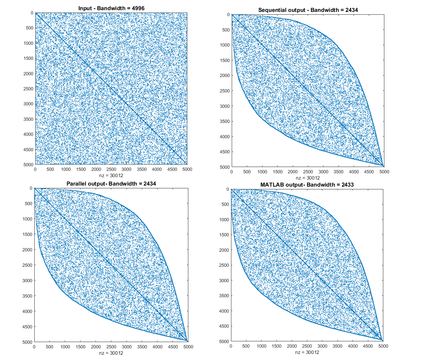
\includegraphics{Webp.net-resizeimage (2).jpg}
    \caption{Validation Benchmark}
    \label{fig:validation}
\end{figure}

\subsection{Execution Time Test}
Execution time benchmarking was performed on a DELL laptop with an Intel® Core™ i7-6500U CPU @ 2.50GHz × 4 processor and 8Gbytes RAM. Also, to test the scalability of our implementation we tested our parallel version on a more powerfull CPU AMD Ryzen7 4700 @ 2.0GHz x 8. Results are depicted in Figure \ref{fig:plot}. The inputs were sparse matrices with variable size and 1\% density. We observed that as density was increasing the speedup among the sequential and parallel implementation was also increasing. This is a reasonable observation, as a more dense matrix means that a node has more neighbours and as a result there are more iterations in the for loops that can be parallelized.
\begin{figure}[H]
    \centering
    %% Creator: Matplotlib, PGF backend
%%
%% To include the figure in your LaTeX document, write
%%   \input{<filename>.pgf}
%%
%% Make sure the required packages are loaded in your preamble
%%   \usepackage{pgf}
%%
%% Figures using additional raster images can only be included by \input if
%% they are in the same directory as the main LaTeX file. For loading figures
%% from other directories you can use the `import` package
%%   \usepackage{import}
%% and then include the figures with
%%   \import{<path to file>}{<filename>.pgf}
%%
%% Matplotlib used the following preamble
%%   \usepackage{fontspec}
%%   \setmainfont{DejaVuSerif.ttf}[Path=/home/evangelos/anaconda3/lib/python3.7/site-packages/matplotlib/mpl-data/fonts/ttf/]
%%   \setsansfont{DejaVuSans.ttf}[Path=/home/evangelos/anaconda3/lib/python3.7/site-packages/matplotlib/mpl-data/fonts/ttf/]
%%   \setmonofont{DejaVuSansMono.ttf}[Path=/home/evangelos/anaconda3/lib/python3.7/site-packages/matplotlib/mpl-data/fonts/ttf/]
%%
\begingroup%
\makeatletter%
\begin{pgfpicture}%
\pgfpathrectangle{\pgfpointorigin}{\pgfqpoint{6.590000in}{3.330000in}}%
\pgfusepath{use as bounding box, clip}%
\begin{pgfscope}%
\pgfsetbuttcap%
\pgfsetmiterjoin%
\definecolor{currentfill}{rgb}{1.000000,1.000000,1.000000}%
\pgfsetfillcolor{currentfill}%
\pgfsetlinewidth{0.000000pt}%
\definecolor{currentstroke}{rgb}{1.000000,1.000000,1.000000}%
\pgfsetstrokecolor{currentstroke}%
\pgfsetdash{}{0pt}%
\pgfpathmoveto{\pgfqpoint{0.000000in}{0.000000in}}%
\pgfpathlineto{\pgfqpoint{6.590000in}{0.000000in}}%
\pgfpathlineto{\pgfqpoint{6.590000in}{3.330000in}}%
\pgfpathlineto{\pgfqpoint{0.000000in}{3.330000in}}%
\pgfpathclose%
\pgfusepath{fill}%
\end{pgfscope}%
\begin{pgfscope}%
\pgfsetbuttcap%
\pgfsetmiterjoin%
\definecolor{currentfill}{rgb}{1.000000,1.000000,1.000000}%
\pgfsetfillcolor{currentfill}%
\pgfsetlinewidth{0.000000pt}%
\definecolor{currentstroke}{rgb}{0.000000,0.000000,0.000000}%
\pgfsetstrokecolor{currentstroke}%
\pgfsetstrokeopacity{0.000000}%
\pgfsetdash{}{0pt}%
\pgfpathmoveto{\pgfqpoint{0.664028in}{0.582778in}}%
\pgfpathlineto{\pgfqpoint{6.405000in}{0.582778in}}%
\pgfpathlineto{\pgfqpoint{6.405000in}{2.976667in}}%
\pgfpathlineto{\pgfqpoint{0.664028in}{2.976667in}}%
\pgfpathclose%
\pgfusepath{fill}%
\end{pgfscope}%
\begin{pgfscope}%
\pgfpathrectangle{\pgfqpoint{0.664028in}{0.582778in}}{\pgfqpoint{5.740972in}{2.393889in}}%
\pgfusepath{clip}%
\pgfsetroundcap%
\pgfsetroundjoin%
\pgfsetlinewidth{0.803000pt}%
\definecolor{currentstroke}{rgb}{0.800000,0.800000,0.800000}%
\pgfsetstrokecolor{currentstroke}%
\pgfsetdash{}{0pt}%
\pgfpathmoveto{\pgfqpoint{1.399442in}{0.582778in}}%
\pgfpathlineto{\pgfqpoint{1.399442in}{2.976667in}}%
\pgfusepath{stroke}%
\end{pgfscope}%
\begin{pgfscope}%
\definecolor{textcolor}{rgb}{0.150000,0.150000,0.150000}%
\pgfsetstrokecolor{textcolor}%
\pgfsetfillcolor{textcolor}%
\pgftext[x=1.399442in,y=0.485556in,,top]{\color{textcolor}\sffamily\fontsize{10.000000}{12.000000}\selectfont 5000}%
\end{pgfscope}%
\begin{pgfscope}%
\pgfpathrectangle{\pgfqpoint{0.664028in}{0.582778in}}{\pgfqpoint{5.740972in}{2.393889in}}%
\pgfusepath{clip}%
\pgfsetroundcap%
\pgfsetroundjoin%
\pgfsetlinewidth{0.803000pt}%
\definecolor{currentstroke}{rgb}{0.800000,0.800000,0.800000}%
\pgfsetstrokecolor{currentstroke}%
\pgfsetdash{}{0pt}%
\pgfpathmoveto{\pgfqpoint{2.348363in}{0.582778in}}%
\pgfpathlineto{\pgfqpoint{2.348363in}{2.976667in}}%
\pgfusepath{stroke}%
\end{pgfscope}%
\begin{pgfscope}%
\definecolor{textcolor}{rgb}{0.150000,0.150000,0.150000}%
\pgfsetstrokecolor{textcolor}%
\pgfsetfillcolor{textcolor}%
\pgftext[x=2.348363in,y=0.485556in,,top]{\color{textcolor}\sffamily\fontsize{10.000000}{12.000000}\selectfont 10000}%
\end{pgfscope}%
\begin{pgfscope}%
\pgfpathrectangle{\pgfqpoint{0.664028in}{0.582778in}}{\pgfqpoint{5.740972in}{2.393889in}}%
\pgfusepath{clip}%
\pgfsetroundcap%
\pgfsetroundjoin%
\pgfsetlinewidth{0.803000pt}%
\definecolor{currentstroke}{rgb}{0.800000,0.800000,0.800000}%
\pgfsetstrokecolor{currentstroke}%
\pgfsetdash{}{0pt}%
\pgfpathmoveto{\pgfqpoint{3.297284in}{0.582778in}}%
\pgfpathlineto{\pgfqpoint{3.297284in}{2.976667in}}%
\pgfusepath{stroke}%
\end{pgfscope}%
\begin{pgfscope}%
\definecolor{textcolor}{rgb}{0.150000,0.150000,0.150000}%
\pgfsetstrokecolor{textcolor}%
\pgfsetfillcolor{textcolor}%
\pgftext[x=3.297284in,y=0.485556in,,top]{\color{textcolor}\sffamily\fontsize{10.000000}{12.000000}\selectfont 15000}%
\end{pgfscope}%
\begin{pgfscope}%
\pgfpathrectangle{\pgfqpoint{0.664028in}{0.582778in}}{\pgfqpoint{5.740972in}{2.393889in}}%
\pgfusepath{clip}%
\pgfsetroundcap%
\pgfsetroundjoin%
\pgfsetlinewidth{0.803000pt}%
\definecolor{currentstroke}{rgb}{0.800000,0.800000,0.800000}%
\pgfsetstrokecolor{currentstroke}%
\pgfsetdash{}{0pt}%
\pgfpathmoveto{\pgfqpoint{4.246205in}{0.582778in}}%
\pgfpathlineto{\pgfqpoint{4.246205in}{2.976667in}}%
\pgfusepath{stroke}%
\end{pgfscope}%
\begin{pgfscope}%
\definecolor{textcolor}{rgb}{0.150000,0.150000,0.150000}%
\pgfsetstrokecolor{textcolor}%
\pgfsetfillcolor{textcolor}%
\pgftext[x=4.246205in,y=0.485556in,,top]{\color{textcolor}\sffamily\fontsize{10.000000}{12.000000}\selectfont 20000}%
\end{pgfscope}%
\begin{pgfscope}%
\pgfpathrectangle{\pgfqpoint{0.664028in}{0.582778in}}{\pgfqpoint{5.740972in}{2.393889in}}%
\pgfusepath{clip}%
\pgfsetroundcap%
\pgfsetroundjoin%
\pgfsetlinewidth{0.803000pt}%
\definecolor{currentstroke}{rgb}{0.800000,0.800000,0.800000}%
\pgfsetstrokecolor{currentstroke}%
\pgfsetdash{}{0pt}%
\pgfpathmoveto{\pgfqpoint{5.195126in}{0.582778in}}%
\pgfpathlineto{\pgfqpoint{5.195126in}{2.976667in}}%
\pgfusepath{stroke}%
\end{pgfscope}%
\begin{pgfscope}%
\definecolor{textcolor}{rgb}{0.150000,0.150000,0.150000}%
\pgfsetstrokecolor{textcolor}%
\pgfsetfillcolor{textcolor}%
\pgftext[x=5.195126in,y=0.485556in,,top]{\color{textcolor}\sffamily\fontsize{10.000000}{12.000000}\selectfont 25000}%
\end{pgfscope}%
\begin{pgfscope}%
\pgfpathrectangle{\pgfqpoint{0.664028in}{0.582778in}}{\pgfqpoint{5.740972in}{2.393889in}}%
\pgfusepath{clip}%
\pgfsetroundcap%
\pgfsetroundjoin%
\pgfsetlinewidth{0.803000pt}%
\definecolor{currentstroke}{rgb}{0.800000,0.800000,0.800000}%
\pgfsetstrokecolor{currentstroke}%
\pgfsetdash{}{0pt}%
\pgfpathmoveto{\pgfqpoint{6.144047in}{0.582778in}}%
\pgfpathlineto{\pgfqpoint{6.144047in}{2.976667in}}%
\pgfusepath{stroke}%
\end{pgfscope}%
\begin{pgfscope}%
\definecolor{textcolor}{rgb}{0.150000,0.150000,0.150000}%
\pgfsetstrokecolor{textcolor}%
\pgfsetfillcolor{textcolor}%
\pgftext[x=6.144047in,y=0.485556in,,top]{\color{textcolor}\sffamily\fontsize{10.000000}{12.000000}\selectfont 30000}%
\end{pgfscope}%
\begin{pgfscope}%
\definecolor{textcolor}{rgb}{0.150000,0.150000,0.150000}%
\pgfsetstrokecolor{textcolor}%
\pgfsetfillcolor{textcolor}%
\pgftext[x=3.534514in,y=0.295587in,,top]{\color{textcolor}\sffamily\fontsize{10.000000}{12.000000}\selectfont Size - n}%
\end{pgfscope}%
\begin{pgfscope}%
\pgfpathrectangle{\pgfqpoint{0.664028in}{0.582778in}}{\pgfqpoint{5.740972in}{2.393889in}}%
\pgfusepath{clip}%
\pgfsetroundcap%
\pgfsetroundjoin%
\pgfsetlinewidth{0.803000pt}%
\definecolor{currentstroke}{rgb}{0.800000,0.800000,0.800000}%
\pgfsetstrokecolor{currentstroke}%
\pgfsetdash{}{0pt}%
\pgfpathmoveto{\pgfqpoint{0.664028in}{0.676500in}}%
\pgfpathlineto{\pgfqpoint{6.405000in}{0.676500in}}%
\pgfusepath{stroke}%
\end{pgfscope}%
\begin{pgfscope}%
\definecolor{textcolor}{rgb}{0.150000,0.150000,0.150000}%
\pgfsetstrokecolor{textcolor}%
\pgfsetfillcolor{textcolor}%
\pgftext[x=0.345926in,y=0.623738in,left,base]{\color{textcolor}\sffamily\fontsize{10.000000}{12.000000}\selectfont 0.0}%
\end{pgfscope}%
\begin{pgfscope}%
\pgfpathrectangle{\pgfqpoint{0.664028in}{0.582778in}}{\pgfqpoint{5.740972in}{2.393889in}}%
\pgfusepath{clip}%
\pgfsetroundcap%
\pgfsetroundjoin%
\pgfsetlinewidth{0.803000pt}%
\definecolor{currentstroke}{rgb}{0.800000,0.800000,0.800000}%
\pgfsetstrokecolor{currentstroke}%
\pgfsetdash{}{0pt}%
\pgfpathmoveto{\pgfqpoint{0.664028in}{0.983105in}}%
\pgfpathlineto{\pgfqpoint{6.405000in}{0.983105in}}%
\pgfusepath{stroke}%
\end{pgfscope}%
\begin{pgfscope}%
\definecolor{textcolor}{rgb}{0.150000,0.150000,0.150000}%
\pgfsetstrokecolor{textcolor}%
\pgfsetfillcolor{textcolor}%
\pgftext[x=0.345926in,y=0.930343in,left,base]{\color{textcolor}\sffamily\fontsize{10.000000}{12.000000}\selectfont 0.5}%
\end{pgfscope}%
\begin{pgfscope}%
\pgfpathrectangle{\pgfqpoint{0.664028in}{0.582778in}}{\pgfqpoint{5.740972in}{2.393889in}}%
\pgfusepath{clip}%
\pgfsetroundcap%
\pgfsetroundjoin%
\pgfsetlinewidth{0.803000pt}%
\definecolor{currentstroke}{rgb}{0.800000,0.800000,0.800000}%
\pgfsetstrokecolor{currentstroke}%
\pgfsetdash{}{0pt}%
\pgfpathmoveto{\pgfqpoint{0.664028in}{1.289709in}}%
\pgfpathlineto{\pgfqpoint{6.405000in}{1.289709in}}%
\pgfusepath{stroke}%
\end{pgfscope}%
\begin{pgfscope}%
\definecolor{textcolor}{rgb}{0.150000,0.150000,0.150000}%
\pgfsetstrokecolor{textcolor}%
\pgfsetfillcolor{textcolor}%
\pgftext[x=0.345926in,y=1.236948in,left,base]{\color{textcolor}\sffamily\fontsize{10.000000}{12.000000}\selectfont 1.0}%
\end{pgfscope}%
\begin{pgfscope}%
\pgfpathrectangle{\pgfqpoint{0.664028in}{0.582778in}}{\pgfqpoint{5.740972in}{2.393889in}}%
\pgfusepath{clip}%
\pgfsetroundcap%
\pgfsetroundjoin%
\pgfsetlinewidth{0.803000pt}%
\definecolor{currentstroke}{rgb}{0.800000,0.800000,0.800000}%
\pgfsetstrokecolor{currentstroke}%
\pgfsetdash{}{0pt}%
\pgfpathmoveto{\pgfqpoint{0.664028in}{1.596314in}}%
\pgfpathlineto{\pgfqpoint{6.405000in}{1.596314in}}%
\pgfusepath{stroke}%
\end{pgfscope}%
\begin{pgfscope}%
\definecolor{textcolor}{rgb}{0.150000,0.150000,0.150000}%
\pgfsetstrokecolor{textcolor}%
\pgfsetfillcolor{textcolor}%
\pgftext[x=0.345926in,y=1.543553in,left,base]{\color{textcolor}\sffamily\fontsize{10.000000}{12.000000}\selectfont 1.5}%
\end{pgfscope}%
\begin{pgfscope}%
\pgfpathrectangle{\pgfqpoint{0.664028in}{0.582778in}}{\pgfqpoint{5.740972in}{2.393889in}}%
\pgfusepath{clip}%
\pgfsetroundcap%
\pgfsetroundjoin%
\pgfsetlinewidth{0.803000pt}%
\definecolor{currentstroke}{rgb}{0.800000,0.800000,0.800000}%
\pgfsetstrokecolor{currentstroke}%
\pgfsetdash{}{0pt}%
\pgfpathmoveto{\pgfqpoint{0.664028in}{1.902919in}}%
\pgfpathlineto{\pgfqpoint{6.405000in}{1.902919in}}%
\pgfusepath{stroke}%
\end{pgfscope}%
\begin{pgfscope}%
\definecolor{textcolor}{rgb}{0.150000,0.150000,0.150000}%
\pgfsetstrokecolor{textcolor}%
\pgfsetfillcolor{textcolor}%
\pgftext[x=0.345926in,y=1.850158in,left,base]{\color{textcolor}\sffamily\fontsize{10.000000}{12.000000}\selectfont 2.0}%
\end{pgfscope}%
\begin{pgfscope}%
\pgfpathrectangle{\pgfqpoint{0.664028in}{0.582778in}}{\pgfqpoint{5.740972in}{2.393889in}}%
\pgfusepath{clip}%
\pgfsetroundcap%
\pgfsetroundjoin%
\pgfsetlinewidth{0.803000pt}%
\definecolor{currentstroke}{rgb}{0.800000,0.800000,0.800000}%
\pgfsetstrokecolor{currentstroke}%
\pgfsetdash{}{0pt}%
\pgfpathmoveto{\pgfqpoint{0.664028in}{2.209524in}}%
\pgfpathlineto{\pgfqpoint{6.405000in}{2.209524in}}%
\pgfusepath{stroke}%
\end{pgfscope}%
\begin{pgfscope}%
\definecolor{textcolor}{rgb}{0.150000,0.150000,0.150000}%
\pgfsetstrokecolor{textcolor}%
\pgfsetfillcolor{textcolor}%
\pgftext[x=0.345926in,y=2.156762in,left,base]{\color{textcolor}\sffamily\fontsize{10.000000}{12.000000}\selectfont 2.5}%
\end{pgfscope}%
\begin{pgfscope}%
\pgfpathrectangle{\pgfqpoint{0.664028in}{0.582778in}}{\pgfqpoint{5.740972in}{2.393889in}}%
\pgfusepath{clip}%
\pgfsetroundcap%
\pgfsetroundjoin%
\pgfsetlinewidth{0.803000pt}%
\definecolor{currentstroke}{rgb}{0.800000,0.800000,0.800000}%
\pgfsetstrokecolor{currentstroke}%
\pgfsetdash{}{0pt}%
\pgfpathmoveto{\pgfqpoint{0.664028in}{2.516129in}}%
\pgfpathlineto{\pgfqpoint{6.405000in}{2.516129in}}%
\pgfusepath{stroke}%
\end{pgfscope}%
\begin{pgfscope}%
\definecolor{textcolor}{rgb}{0.150000,0.150000,0.150000}%
\pgfsetstrokecolor{textcolor}%
\pgfsetfillcolor{textcolor}%
\pgftext[x=0.345926in,y=2.463367in,left,base]{\color{textcolor}\sffamily\fontsize{10.000000}{12.000000}\selectfont 3.0}%
\end{pgfscope}%
\begin{pgfscope}%
\pgfpathrectangle{\pgfqpoint{0.664028in}{0.582778in}}{\pgfqpoint{5.740972in}{2.393889in}}%
\pgfusepath{clip}%
\pgfsetroundcap%
\pgfsetroundjoin%
\pgfsetlinewidth{0.803000pt}%
\definecolor{currentstroke}{rgb}{0.800000,0.800000,0.800000}%
\pgfsetstrokecolor{currentstroke}%
\pgfsetdash{}{0pt}%
\pgfpathmoveto{\pgfqpoint{0.664028in}{2.822734in}}%
\pgfpathlineto{\pgfqpoint{6.405000in}{2.822734in}}%
\pgfusepath{stroke}%
\end{pgfscope}%
\begin{pgfscope}%
\definecolor{textcolor}{rgb}{0.150000,0.150000,0.150000}%
\pgfsetstrokecolor{textcolor}%
\pgfsetfillcolor{textcolor}%
\pgftext[x=0.345926in,y=2.769972in,left,base]{\color{textcolor}\sffamily\fontsize{10.000000}{12.000000}\selectfont 3.5}%
\end{pgfscope}%
\begin{pgfscope}%
\definecolor{textcolor}{rgb}{0.150000,0.150000,0.150000}%
\pgfsetstrokecolor{textcolor}%
\pgfsetfillcolor{textcolor}%
\pgftext[x=0.290371in,y=1.779722in,,bottom,rotate=90.000000]{\color{textcolor}\sffamily\fontsize{10.000000}{12.000000}\selectfont Execution Time (seconds)}%
\end{pgfscope}%
\begin{pgfscope}%
\pgfpathrectangle{\pgfqpoint{0.664028in}{0.582778in}}{\pgfqpoint{5.740972in}{2.393889in}}%
\pgfusepath{clip}%
\pgfsetroundcap%
\pgfsetroundjoin%
\pgfsetlinewidth{1.505625pt}%
\definecolor{currentstroke}{rgb}{0.000000,0.501961,0.000000}%
\pgfsetstrokecolor{currentstroke}%
\pgfsetdash{}{0pt}%
\pgfpathmoveto{\pgfqpoint{0.924981in}{0.694570in}}%
\pgfpathlineto{\pgfqpoint{1.399442in}{0.745931in}}%
\pgfpathlineto{\pgfqpoint{1.873902in}{0.817959in}}%
\pgfpathlineto{\pgfqpoint{2.348363in}{0.939310in}}%
\pgfpathlineto{\pgfqpoint{2.822823in}{1.058938in}}%
\pgfpathlineto{\pgfqpoint{3.297284in}{1.225850in}}%
\pgfpathlineto{\pgfqpoint{3.771744in}{1.421004in}}%
\pgfpathlineto{\pgfqpoint{4.246205in}{1.649620in}}%
\pgfpathlineto{\pgfqpoint{4.720665in}{1.910220in}}%
\pgfpathlineto{\pgfqpoint{5.195126in}{2.197716in}}%
\pgfpathlineto{\pgfqpoint{6.144047in}{2.867854in}}%
\pgfusepath{stroke}%
\end{pgfscope}%
\begin{pgfscope}%
\pgfpathrectangle{\pgfqpoint{0.664028in}{0.582778in}}{\pgfqpoint{5.740972in}{2.393889in}}%
\pgfusepath{clip}%
\pgfsetroundcap%
\pgfsetroundjoin%
\pgfsetlinewidth{1.505625pt}%
\definecolor{currentstroke}{rgb}{1.000000,0.000000,0.000000}%
\pgfsetstrokecolor{currentstroke}%
\pgfsetdash{}{0pt}%
\pgfpathmoveto{\pgfqpoint{0.924981in}{0.691591in}}%
\pgfpathlineto{\pgfqpoint{1.399442in}{0.721571in}}%
\pgfpathlineto{\pgfqpoint{1.873902in}{0.763581in}}%
\pgfpathlineto{\pgfqpoint{2.348363in}{0.839960in}}%
\pgfpathlineto{\pgfqpoint{2.822823in}{0.915457in}}%
\pgfpathlineto{\pgfqpoint{3.297284in}{0.997879in}}%
\pgfpathlineto{\pgfqpoint{3.771744in}{1.122401in}}%
\pgfpathlineto{\pgfqpoint{4.246205in}{1.250172in}}%
\pgfpathlineto{\pgfqpoint{4.720665in}{1.412953in}}%
\pgfpathlineto{\pgfqpoint{5.195126in}{1.566571in}}%
\pgfpathlineto{\pgfqpoint{6.144047in}{1.987378in}}%
\pgfusepath{stroke}%
\end{pgfscope}%
\begin{pgfscope}%
\pgfpathrectangle{\pgfqpoint{0.664028in}{0.582778in}}{\pgfqpoint{5.740972in}{2.393889in}}%
\pgfusepath{clip}%
\pgfsetroundcap%
\pgfsetroundjoin%
\pgfsetlinewidth{1.505625pt}%
\definecolor{currentstroke}{rgb}{0.254902,0.411765,0.882353}%
\pgfsetstrokecolor{currentstroke}%
\pgfsetdash{}{0pt}%
\pgfpathmoveto{\pgfqpoint{1.399442in}{0.712679in}}%
\pgfpathlineto{\pgfqpoint{2.348363in}{0.841407in}}%
\pgfpathlineto{\pgfqpoint{3.297284in}{1.036897in}}%
\pgfpathlineto{\pgfqpoint{4.246205in}{1.368807in}}%
\pgfpathlineto{\pgfqpoint{5.195126in}{1.650107in}}%
\pgfpathlineto{\pgfqpoint{6.144047in}{2.104659in}}%
\pgfusepath{stroke}%
\end{pgfscope}%
\begin{pgfscope}%
\pgfpathrectangle{\pgfqpoint{0.664028in}{0.582778in}}{\pgfqpoint{5.740972in}{2.393889in}}%
\pgfusepath{clip}%
\pgfsetroundcap%
\pgfsetroundjoin%
\pgfsetlinewidth{1.505625pt}%
\definecolor{currentstroke}{rgb}{1.000000,0.647059,0.000000}%
\pgfsetstrokecolor{currentstroke}%
\pgfsetdash{}{0pt}%
\pgfpathmoveto{\pgfqpoint{1.399442in}{0.710226in}}%
\pgfpathlineto{\pgfqpoint{2.348363in}{0.778293in}}%
\pgfpathlineto{\pgfqpoint{3.297284in}{0.875180in}}%
\pgfpathlineto{\pgfqpoint{4.246205in}{1.044426in}}%
\pgfpathlineto{\pgfqpoint{5.195126in}{1.068954in}}%
\pgfpathlineto{\pgfqpoint{6.144047in}{1.203860in}}%
\pgfusepath{stroke}%
\end{pgfscope}%
\begin{pgfscope}%
\pgfsetrectcap%
\pgfsetmiterjoin%
\pgfsetlinewidth{0.803000pt}%
\definecolor{currentstroke}{rgb}{0.800000,0.800000,0.800000}%
\pgfsetstrokecolor{currentstroke}%
\pgfsetdash{}{0pt}%
\pgfpathmoveto{\pgfqpoint{0.664028in}{0.582778in}}%
\pgfpathlineto{\pgfqpoint{0.664028in}{2.976667in}}%
\pgfusepath{stroke}%
\end{pgfscope}%
\begin{pgfscope}%
\pgfsetrectcap%
\pgfsetmiterjoin%
\pgfsetlinewidth{0.803000pt}%
\definecolor{currentstroke}{rgb}{0.800000,0.800000,0.800000}%
\pgfsetstrokecolor{currentstroke}%
\pgfsetdash{}{0pt}%
\pgfpathmoveto{\pgfqpoint{6.405000in}{0.582778in}}%
\pgfpathlineto{\pgfqpoint{6.405000in}{2.976667in}}%
\pgfusepath{stroke}%
\end{pgfscope}%
\begin{pgfscope}%
\pgfsetrectcap%
\pgfsetmiterjoin%
\pgfsetlinewidth{0.803000pt}%
\definecolor{currentstroke}{rgb}{0.800000,0.800000,0.800000}%
\pgfsetstrokecolor{currentstroke}%
\pgfsetdash{}{0pt}%
\pgfpathmoveto{\pgfqpoint{0.664028in}{0.582778in}}%
\pgfpathlineto{\pgfqpoint{6.405000in}{0.582778in}}%
\pgfusepath{stroke}%
\end{pgfscope}%
\begin{pgfscope}%
\pgfsetrectcap%
\pgfsetmiterjoin%
\pgfsetlinewidth{0.803000pt}%
\definecolor{currentstroke}{rgb}{0.800000,0.800000,0.800000}%
\pgfsetstrokecolor{currentstroke}%
\pgfsetdash{}{0pt}%
\pgfpathmoveto{\pgfqpoint{0.664028in}{2.976667in}}%
\pgfpathlineto{\pgfqpoint{6.405000in}{2.976667in}}%
\pgfusepath{stroke}%
\end{pgfscope}%
\begin{pgfscope}%
\definecolor{textcolor}{rgb}{0.150000,0.150000,0.150000}%
\pgfsetstrokecolor{textcolor}%
\pgfsetfillcolor{textcolor}%
\pgftext[x=3.534514in,y=3.060000in,,base]{\color{textcolor}\sffamily\fontsize{12.000000}{14.400000}\selectfont Execution Time Benchmark}%
\end{pgfscope}%
\begin{pgfscope}%
\pgfsetbuttcap%
\pgfsetmiterjoin%
\definecolor{currentfill}{rgb}{1.000000,1.000000,1.000000}%
\pgfsetfillcolor{currentfill}%
\pgfsetfillopacity{0.800000}%
\pgfsetlinewidth{1.003750pt}%
\definecolor{currentstroke}{rgb}{0.800000,0.800000,0.800000}%
\pgfsetstrokecolor{currentstroke}%
\pgfsetstrokeopacity{0.800000}%
\pgfsetdash{}{0pt}%
\pgfpathmoveto{\pgfqpoint{0.761250in}{1.846269in}}%
\pgfpathlineto{\pgfqpoint{3.996968in}{1.846269in}}%
\pgfpathquadraticcurveto{\pgfqpoint{4.024746in}{1.846269in}}{\pgfqpoint{4.024746in}{1.874047in}}%
\pgfpathlineto{\pgfqpoint{4.024746in}{2.879444in}}%
\pgfpathquadraticcurveto{\pgfqpoint{4.024746in}{2.907222in}}{\pgfqpoint{3.996968in}{2.907222in}}%
\pgfpathlineto{\pgfqpoint{0.761250in}{2.907222in}}%
\pgfpathquadraticcurveto{\pgfqpoint{0.733472in}{2.907222in}}{\pgfqpoint{0.733472in}{2.879444in}}%
\pgfpathlineto{\pgfqpoint{0.733472in}{1.874047in}}%
\pgfpathquadraticcurveto{\pgfqpoint{0.733472in}{1.846269in}}{\pgfqpoint{0.761250in}{1.846269in}}%
\pgfpathclose%
\pgfusepath{stroke,fill}%
\end{pgfscope}%
\begin{pgfscope}%
\pgfsetroundcap%
\pgfsetroundjoin%
\pgfsetlinewidth{0.000000pt}%
\definecolor{currentstroke}{rgb}{1.000000,1.000000,1.000000}%
\pgfsetstrokecolor{currentstroke}%
\pgfsetdash{}{0pt}%
\pgfpathmoveto{\pgfqpoint{0.789028in}{2.794755in}}%
\pgfpathlineto{\pgfqpoint{1.066806in}{2.794755in}}%
\pgfusepath{}%
\end{pgfscope}%
\begin{pgfscope}%
\definecolor{textcolor}{rgb}{0.150000,0.150000,0.150000}%
\pgfsetstrokecolor{textcolor}%
\pgfsetfillcolor{textcolor}%
\pgftext[x=1.177917in,y=2.746144in,left,base]{\color{textcolor}\sffamily\fontsize{10.000000}{12.000000}\selectfont type}%
\end{pgfscope}%
\begin{pgfscope}%
\pgfsetroundcap%
\pgfsetroundjoin%
\pgfsetlinewidth{1.505625pt}%
\definecolor{currentstroke}{rgb}{0.000000,0.501961,0.000000}%
\pgfsetstrokecolor{currentstroke}%
\pgfsetdash{}{0pt}%
\pgfpathmoveto{\pgfqpoint{0.789028in}{2.590897in}}%
\pgfpathlineto{\pgfqpoint{1.066806in}{2.590897in}}%
\pgfusepath{stroke}%
\end{pgfscope}%
\begin{pgfscope}%
\definecolor{textcolor}{rgb}{0.150000,0.150000,0.150000}%
\pgfsetstrokecolor{textcolor}%
\pgfsetfillcolor{textcolor}%
\pgftext[x=1.177917in,y=2.542286in,left,base]{\color{textcolor}\sffamily\fontsize{10.000000}{12.000000}\selectfont sequential intel i7 @ 2.5GHz x 4}%
\end{pgfscope}%
\begin{pgfscope}%
\pgfsetroundcap%
\pgfsetroundjoin%
\pgfsetlinewidth{1.505625pt}%
\definecolor{currentstroke}{rgb}{1.000000,0.000000,0.000000}%
\pgfsetstrokecolor{currentstroke}%
\pgfsetdash{}{0pt}%
\pgfpathmoveto{\pgfqpoint{0.789028in}{2.387040in}}%
\pgfpathlineto{\pgfqpoint{1.066806in}{2.387040in}}%
\pgfusepath{stroke}%
\end{pgfscope}%
\begin{pgfscope}%
\definecolor{textcolor}{rgb}{0.150000,0.150000,0.150000}%
\pgfsetstrokecolor{textcolor}%
\pgfsetfillcolor{textcolor}%
\pgftext[x=1.177917in,y=2.338429in,left,base]{\color{textcolor}\sffamily\fontsize{10.000000}{12.000000}\selectfont parallel intel i7 @ 2.5GHz x 4}%
\end{pgfscope}%
\begin{pgfscope}%
\pgfsetroundcap%
\pgfsetroundjoin%
\pgfsetlinewidth{1.505625pt}%
\definecolor{currentstroke}{rgb}{0.254902,0.411765,0.882353}%
\pgfsetstrokecolor{currentstroke}%
\pgfsetdash{}{0pt}%
\pgfpathmoveto{\pgfqpoint{0.789028in}{2.183183in}}%
\pgfpathlineto{\pgfqpoint{1.066806in}{2.183183in}}%
\pgfusepath{stroke}%
\end{pgfscope}%
\begin{pgfscope}%
\definecolor{textcolor}{rgb}{0.150000,0.150000,0.150000}%
\pgfsetstrokecolor{textcolor}%
\pgfsetfillcolor{textcolor}%
\pgftext[x=1.177917in,y=2.134572in,left,base]{\color{textcolor}\sffamily\fontsize{10.000000}{12.000000}\selectfont MATLAB intel i7 @ 2.5GHz x 4}%
\end{pgfscope}%
\begin{pgfscope}%
\pgfsetroundcap%
\pgfsetroundjoin%
\pgfsetlinewidth{1.505625pt}%
\definecolor{currentstroke}{rgb}{1.000000,0.647059,0.000000}%
\pgfsetstrokecolor{currentstroke}%
\pgfsetdash{}{0pt}%
\pgfpathmoveto{\pgfqpoint{0.789028in}{1.979326in}}%
\pgfpathlineto{\pgfqpoint{1.066806in}{1.979326in}}%
\pgfusepath{stroke}%
\end{pgfscope}%
\begin{pgfscope}%
\definecolor{textcolor}{rgb}{0.150000,0.150000,0.150000}%
\pgfsetstrokecolor{textcolor}%
\pgfsetfillcolor{textcolor}%
\pgftext[x=1.177917in,y=1.930715in,left,base]{\color{textcolor}\sffamily\fontsize{10.000000}{12.000000}\selectfont parallel AMD Ryzen7 4700U @ 2GHz x 8}%
\end{pgfscope}%
\end{pgfpicture}%
\makeatother%
\endgroup%

    \caption{Execution Time Benchmark}
    \label{fig:plot}
\end{figure}


\end{document}
